\title{Vectors in $\mathbb R^n$} 
\subtitle{\SubTitleName}
\institute[]{\Course}
\author{\Instructor}
\maketitle   




\frame{\frametitle{Topics and Learning Objectives}

\Emph{Topics} \\
\TopicStatement

\begin{itemize}
    \item  vectors in $ \mathbb R ^{n}$, and their basic properties 
    
    % \item  Linear combinations of vectors 

\end{itemize}

\vspace{0.5cm}

\LO\\

\LearningObjectiveStatement

\begin{itemize}
    \item  apply geometric and algebraic properties of vectors in $ \mathbb R ^{n}$ to compute vector additions and scalar multiplications
    % \item  Characterize a set of vectors in terms of \Emph{linear combinations}, their \Emph{span}, and how they are related to each other geometrically.
\end{itemize}



}



\begin{frame}{Motivation}

    We want to think about the \Emph{algebra} in linear algebra (systems of
    equations and their solution sets) in terms of \Emph{geometry} (points, lines,
    planes, etc).
    
    \pause 
    \vspace{12pt}
    
        \begin{minipage}{.52\textwidth}
    
    %\def\r{\color{DarkRed}}\def\b{\color{Teal}}
        \begin{align*} 
            \color{DarkRed} x - 3y & \color{DarkRed} = -3\\
            \color{Teal} 2x + y & \color{Teal} = 8 
        \end{align*}
    
            \end{minipage} \begin{minipage}{.46\textwidth}
    
     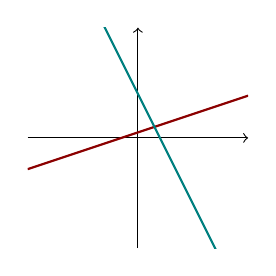
\begin{tikzpicture}[scale=.07, baseline]
    %   \draw (-20,-20) rectangle (20,20);
      \clip (-20,-20) rectangle (20,20);
      \draw[->] (-20,0) -- (20,0);
      \draw[->] (0,-20) -- (0,20);
      \draw[DarkRed, thick] (-20,-20/3+1) -- (20,20/3+1);
      \draw[Teal, thick] (-20,40+8) -- (20,-40+8);
      %\point at (3,2);
    \end{tikzpicture}
        \end{minipage} 
    
    \vspace{12pt}
    
    This other perspective:
    \begin{itemize}
        \item gives us deeper insight into the properties of systems and their solutions
        \item requires that we introduce $n$-dimensional space $\R^n$, and
    \Emph{vectors} inside it.
    \end{itemize}


\end{frame}





\begin{frame}
\frametitle{Definition of $\R^n$}

    $\R$ denotes the collection of all real numbers.\\[12pt]

    \pause 
    Let $n$ be a positive whole number.  We define
    \[ \R^n = \text{all ordered } n\text{-tuples of real numbers }
    (x_1,\,x_2,\,x_3,\,\ldots,\,x_n). \]

    \pause 

  When $n=1$, we get $\R$ back: $\R^1 = \R$. Geometrically, this is the
  \Emph{number line}.
  \begin{center}
    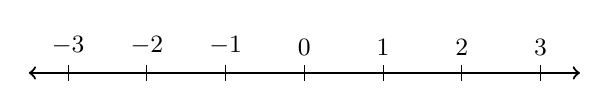
\begin{tikzpicture}
      \draw [<->, thick] (-3.5,0) -- (3.5,0);
      \foreach \x in {-3,...,3}
         \draw[thin] (\x,-.1) -- (\x,0.1) node[anchor=south] {\small$\x$};
    \end{tikzpicture}
  \end{center}

\end{frame}



\begin{frame}{Definition of $\R^2$}

    \vskip-1mm
    Note that:
    \begin{itemize}
    \item when $n=2$, we can think of $\R^2$ as a \Emph{plane}
    \item every point in this plane can be represented by an ordered pair of real numbers, its $x$- and $y$-coordinates
    \end{itemize}
  \vskip .5cm
  \pause 
  \Emph{Example}: Sketch the point $(3,2)$ and the vector $\spalignmat{3;2}$.
  \begin{center}
    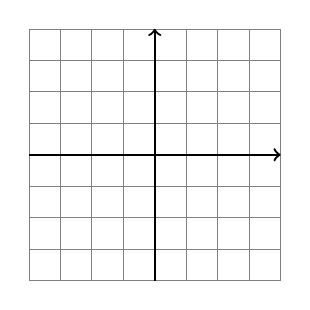
\begin{tikzpicture}[scale=.4]%[every node/.append, %style={whitebg, thin border},
       % every label/.append style={text=seq-blue}, scale=.5]
      \draw[help lines] (-4, -4) grid (4, 4);
      \draw[->, thick] (-4,0) -- (4,0);
      \draw[->, thick] (0,-4) -- (0,4);
      %\point[blue] at (1,2);
      %\point[blue] at (0,-3);
    \end{tikzpicture}
  \end{center}

\end{frame}



\begin{frame}
\frametitle{Vectors as Points in $\mathbb R^n$}
    In the previous slides, we were thinking of elements of $\R^n$ as
    \Emph{points}: in the line, plane, space, etc.

    \vspace{12pt}
    \pause 
    We can also think of them as \Emph{vectors}: arrows with a given length and
    direction. 
    \pause 
\begin{center}
    \begin{tikzpicture}[scale=0.5] % every pin/.style={whitebg, thin border}]
      %\draw[grid lines] (-1,-1) grid (4, 4);
      \draw[->, thick] (-1,0) -- (4,0);
      \draw[->, thick] (0,-1) -- (0,4);
      %\point[blue, pin={
          %[pin edge={Teal}, text=blue, right]
          %10:the point $(1,3)$}] (x) at (1,3);

    \end{tikzpicture}
\end{center}

    For example, the vector $\spalignmat{3;2}$ points \Emph{horizontally} in the amount of its $x$-coordinate,
and \Emph{vertically} in the amount of its $y$-coordinate.

\end{frame}





\frame{\frametitle{Vector Algebra}

    When we think of an element of $\R^n$ as a vector, we write it as a matrix with
    $n$ rows and one column. \pause For example, suppose 
    \begin{equation*}
        \vec u = \spalignmat{ u_1 ; u_2 },
        \quad
        \vec v = \spalignmat{ v_1 ; v_2 }.
    \end{equation*}
    
    \pause 
    Vectors have the following properties.

    \begin{enumerate}
        \item \Emph{Scalar Multiples}:  $$ c \vec u = \spalignmat{cu_1;cu_2}$$
        
        \item \Emph{Vector Addition}: 
        \begin{equation*}
        \vec u + \vec v = \spalignmat{u_1+v_1;u_2+v_2}
        \end{equation*}
    \end{enumerate}
    
    \vspace{12pt} 
    \pause 
    Note that vectors in higher dimensions have the same properties. 

}

\frame{\frametitle{Parallelogram Rule for Vector Addition}
  \begin{center}
        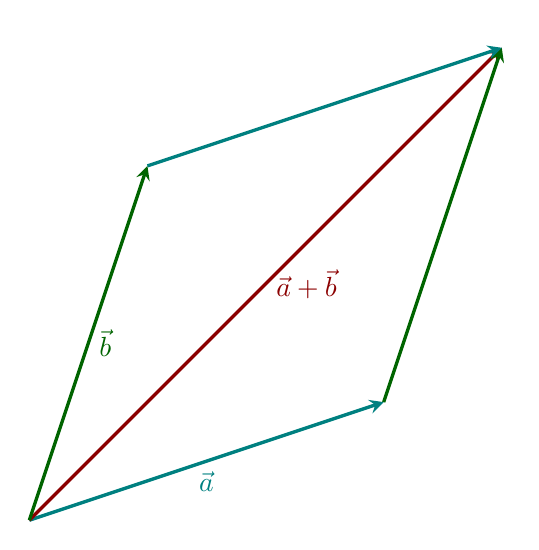
\begin{tikzpicture}[scale=0.5] 
            \draw[->,Teal,very thick,-stealth] (0,0) -- (9,3) node[midway,below] {$\vec a$};
            \draw[->,DarkRed,very thick,-stealth] (0,0) -- (12,12) node[midway, right] {$\vec a+\vec b$}; 
            \draw[->,DarkGreen,very thick,-stealth] (0,0) -- (3,9) node[midway, right] {$\vec b$};
            
             \draw[->,DarkGreen,very thick,-stealth] (9,3) -- (12,12) node[above] {}; 
            \draw[->,Teal,very thick,-stealth] (3,9) -- (12,12) node[above] {};           
        \end{tikzpicture}
    \end{center}
    
    
}


\frame{\frametitle{Summary}

We explored the following concepts in this video. \vspace{4pt}
\begin{itemize}\setlength{\itemsep}{8pt}
    \item geometric and algebraic properties of vectors in $ \mathbb R ^{n}$ 
    \item vector algebra: compute vector additions and scalar multiplications
\end{itemize}

}
